%
% Qualitative example of switch bouncing versus CPU clock.
%
\documentclass[border=3mm]{standalone}
\usepackage{tikz}
\usetikzlibrary{circuits.ee.IEC}

\begin{document}

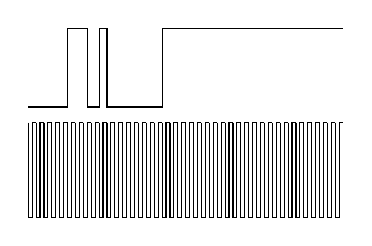
\begin{tikzpicture}
    \draw [-] (0,0)
        to (0.5,0) to (0.5,1)
        to (0.75,1) to (0.75,0)
        to (0.9,0) to (0.9,1)
        to (1.0,1) to (1.0,0)
        to (1.7,0) to (1.7,1)
        to (4,1);
    \foreach \x [evaluate=\x as \inieval using 2*\x] in {0,0.05,...,2}
        \draw[thin] (\inieval,-0.2) -- ++(0,-1.2) -| (\inieval+0.05,-0.2) -- (\inieval+0.1,-0.2);
\end{tikzpicture}

\end{document}

